\documentclass[a4j,12pt]{article}
\usepackage[dvipdfmx]{graphicx}

\usepackage[top=3cm, bottom=3cm, left=2.5cm, right=2.5cm]{geometry}
\usepackage{amsmath}
\usepackage{autobreak}

\usepackage{booktabs,caption}
\usepackage[flushleft]{threeparttable}

\setlength{\parindent}{4em}
\setlength{\parskip}{1em}
%\renewcommand{\baselinestretch}{2.0} # Double Space

\title{Acquisition of Microfinance Institutions}
\author{Daiju Aiba \\
        \small JICA Ogata Research Institute 
        \thanks{This paper is part of the project "The Study on the Promotion of Financial Inclusion in Cambodia" by the JICA Ogata Sadako Research Institute for Peace and Development. The project is partially financially supported by Grant-in-Aid for Scientific Research (C) Grants No. 18K01641. The authors also acknowledge significant support by the Cambodia Microfinance Association. }\\
}

\date{\today}

\providecommand{\keywords}[1]
{
  \small	
  \textbf{\textit{Keywords---}} #1
}




\begin{document}
\maketitle


\begin{abstract}
  While the recent flourishment of the microfinance sector attracted the large inflow of capital investment into it, there has been an increasing number of acquisition cases of microfinance institutions by domestic commercial banks and foreign private companies. This study investigates the situation of the recent capital inflow into the Cambodian microfinance sector, and also examines the impact of the recent acquisition of microfinance institutions in Cambodia. 
\keywords{Microfinance Institutions, Financial Inclusion, SDG Investment, Capital Inflow}
\end{abstract} 
  
\section{Introduction}

In recent years, microfinance institutions (MFIs) have played an important role in poverty alleviaition through financial inclusion for developing countries. Along with the recent prosperity of MFIs, there are also a flood of capital inflow into them. The capital inflow takes various forms, such as debt and equity investment, and there exist a variety of investors and lenders. According to El-Zoghbi (2011) and Reille et al. (2011), those investors could be categorized into:
- Individuals
- Retail investors (Such as Oikocredit (Netherlands), responsAbility (Switzerland)), 
	- Retail investors represent 16 percent of the total stock of cross-border funding (Rellie et al., 2011).
- Institutional investors (Commercial banks, insurance companies, pension funds, private  firms, and other corporate companies.)
- Development financial institutions (such as AECID, EBRD, IFC, KfW, and OPIC)      
    - The development financial institutions could be further divided into bilateral and multilateral entities.

 Generally, retail investors have big social goals. Although retail investor demand for microfinance is strong, its growth has been hampered by financial market regulations that do not allow microfinance investment funds distribution to the retail market in the United States and Europe (Rellie et al., 2011). Institutional investors are usually attracted by three features of microfinance, namely its social value, its perceived attractive risk-adjusted returns, and its potential negative correlation from other asset classes. Capital inflows from those investors have assisted the evolution of MFIs in developing countries.

In the meantime, there are several concerns of recent capital inflow into MFIs. Although capital inflows into MFIs have assisted financial inclusion, it could also encourage commercialization of MFIs and even foster mission drift. Particularly, mergers and acquisitions (M\&A) of MFIs by private institutional investors have increased rapidly in recent years. Through M\&A, the ownership and governance mechanism of MFIs could be severely changed. Thus, the objective of the MFIs could be distorted after the M\&A cases.


In this study, we aim to empirically estimate the effect of M\&A cases of MFIs on MFI lending behavior, such as amounts of outstanding loans, and loan size per borrower, the total number of borrowers, and the ratio of female borrowers. For this purpose, we use a difference-in-difference approach and employ the detailed data of MFI lending at MFI-district pair data from Cambodia Microfinance Association.


\section{The Microfinance Sector and Recent Acquisition}
\subsection{Literature of Merger \& Acquisition of Financial Institutions }
There has been a strand of literature of Merger \& Acquisition in a banking sector (Asimakopoulos et al, 2013). The main motives of mergers are to achieve the economies of scale and scope, and to gain access to large client base and to diversify the income sources particularly in cross-border M\&A cases (Asimakopoulos et al, 2013). In the meantime, there is also risks of M\&A. If the cultural differences are serious between acquired financial institutions and target financial institutions, M\&A could cause inefficiency in operation, and lower the performance of a targeted financial institution.


xx (2005) has studied the entry of foreign banks in developing country, and they documented evidence that the form of entry matters to the efficiency of foreign banks. He showed that takeover of domestic banks exhibits higher efficiency than greenfield entry.

In a microfinance sector, there has been an increasing number of M\&A cases in recent decades. In Peru, M\&A activities began in 2006 when Edyficar acquired Crear Cusco to expand its client outreach. M\&A cases continued among several institutions. Later, commercial banks, including BBVA, Scotiabank, and BCP also showed strategic interest on the MFIs. [3]   In Tanzania, three banks; Mwanga Community Bank, Hakika Microfinance Bank, and EFC Microfinance Bank have merged in Tanzania. The Bank of Tanzania approved the formation of the Mwanga Hakika Microfinance Bank on January 2020, and later licensed it on July 2020. The motive for the merger was to enhance compliance, efficiency, and performance while providing financial services to individuals, MSMEs, and corporate clients.[1]
Furthermore, the central bank of Nepal, Nepal Rastra Bank, promotes M\&A of MFIs to strengthen the paid-up capital and ensure reliable financial services. As a result, the central bank plans to reduce the number of MFIs from 84 to 30, and also to increase the minimum paid-up capital of them. For the state- and national-level microfinance companies, the required paid-up capitals are 10 and 100 million Rs, respectively. The central bank provides incentives to the merged/acquired ones through permitting them to issue their right shares. Moreover, the recent coronavirus pandemic made most of the MFIs to opt for M\&A to strengthen their capital. As of May 2021, 28 microfinance companies have completed M\&A and formed 13 micro-financial institutions. Additionally, those entered into M\&A agreement include 35 microfinance companies, consolidating into 17 MFIs[2]


\subsection{Microfinance Institutions and Acquisition in Cambodia}
In Cambodia, there have been 81 microfinance institutions, including six microfinance deposit-taking institutions at the end of 2020. The National Bank of Cambodia (NBC) put several regulations to facilitate and monitor the operations of microfinance institutions and other financial institutions. Also, NBC has been revising several of such regulations recently. Some of these revisions include the modifications in the minimum capital requirement, independency of management, net-worth computation, liquidity coverage ratio, solvency ratio, capital buffer, and interest rate ceilings, among others.   

Before 2000, the microfinance sector includes about 370,651 clients in 2001, representing 17 percent of all households and 29.3 million USD loans outstanding. The major service providers include ACLEDA, PRASAC, EMT, CRS/TCP, and CCB. The market leaders, ACLEDA and EMT, represent 36 and 64 percent of clients and loans outstanding. The National Bank of Cambodia made the registration and licensing of entities providing credit and savings activities. These include preparing the law on Banking and Financial Institutions on November 18, 1999, and the statute on the licensing of Specialized Banking Institutions (SBIs) and Microfinance Institutions (MFIs).[3]  

In recent years,  there has been an increasing number of M\&A cases in the Cambodian microfinance sector. [4] Most are cross-border M\&A by foreign financial institutions. For example, in 2014, Sathapana Microfinance, which was established in 2000s and one of the largest MFIs in Cambodia, were acquired by Maruhan Japan Bank, which was a Japanese-owned commercial banks. In 2016, Sathapana  Microfinance was merged with Maruhan Japan Bank, and transformed into a commercial bank.  In other cases, in 2018, AMK was acquired by Shanghai Commercial \& Savings Bank, which is currently based in Taiwan. In 2017, the Bank of East Asia (Hongkong) and Sri Lanka’s LOLC  jointly acquired a majority stake in Prasac Microfinance, the Cambodia’s largest MFI. In 2018, SAMIC Microfinance was acquired by NongHyup Bank in South Korea, and changed its name to NongHyup Finance.  

As argued by Vanroose and D'Espallier (2013), outreach and operations of MFIs were determined by the development of traditional financial institutions, such as commercial banks.The lower the development of tranditional financial institions, MFIs are more likely to be outreach-oriented and have larger operation. In the case of Camnbodia, traditional banking sector were underdeveloped when NBC started to promote commercilization of the MFIs (Aiba and Okuda, 2020). In recent years, most of the indivdual loans are disbursed by MFIs, meaning that Cambodian MFIs have significant share in retail banking (Aiba et al, 2021). Thus, cross-border M\&A is often aimed to gain the large customer basis and enter the Cambodian market.  

Major challenges of MFIs in Cambodia include the exclusion of the poorest of the poor from the primary target of the institutions, difficulty in reaching the poorest of the poor in the remote rural areas, the high competitive interest rates offered by the MFIs in Cambodia, managing risks of their operations, and the rapidly increasing multiple lending taken by borrowers (Tahir and Tahrim, 2015). M\&A could help MFIs improve their operation by achieving the economies of scale and scope, and by consolidating planning and management information and financial administrations systems. However, the recent M\&A cases are mainly cross-border M\&A, aiming to enter the Cambodian financial market. Thus, there are concerns of mission drift by changes in board structure and management schemes, and inefficiency could occur due to cultural difference.


\section{Empirical Methodology} 
\subsection{Empirical Model}
We use difference-in-difference approach for estimating the impact of acquisition cases. Specifically, we use the following specification for the estimation. 


\begin{equation}
     y_{ijt} = \Sigma_{k=-4}^{-1} \beta_{k} \times treat_{ik} + \Sigma_{k=0}^{4} \beta_{k} \times treat_{ik}+\gamma X_{it} + \mu_i+\nu_{jt} + \epsilon_{ijt} 
\end{equation}

$treat_{ik}$ is a dummy variable taking one if the period relative to first treated period is the same value as k; 0 otherwise, and it also takes 0 for all never-treated groups. Estimation is performed with standard errors clustered at a district level.  

 We also include the time-variant district-level fixed effect, $\nu_{jt}$. Khwaja and Mian (2008) developed the model to include the time-variant district-specific effect. This term controls the effects caused by district-level demand shocks, such as natural disasters, and economic development.  

 To confirm whether the data supports the parallel trends assumption in DID estimation, we also examine whether the control and treated groups have statistically the same trends before treatment. The coefficients $\beta_{k}$ for $k<0$ capture the trends of difference between treatment and control groups before the treatment. The parallel trend assumption holds if $\beta_{k} - \Sigma_{k=-4}^{-1}\beta_k$ statistically equals zero for $k<0$. 
 
Furthermore, we also examine the heterogenious impact of the acquisition cases. The acquisition cases could drive MFIs from a poverty alleviation mission, and could increase loan provision to developed areas. To examine such changes in MFI lending behavior, we include the interaction terms of the treatment dummy with indicators of economic development. Specifically, we extend the model to the following specification.  


\begin{align}
  \begin{autobreak}
    y_{ijt} 
      =  \Sigma_{k=-4}^{-1} \beta_{k} \times treat_{ik} + \Sigma_{k=0}^{4} \beta_{k} \times treat_{ik} +  \Sigma_{k=-4}^{-1} \delta_{k} \times treat_{ik} \times  PopDensity_{jt} 
        +\Sigma_{k=0}^{4} \delta_{k} \times treat_{ik} \times  PopDensity_{jt} + \gamma X_{it} + \mu_i + \nu_{jt} + \epsilon_{ijt} 
  \end{autobreak}
\end{align}


where $PopDensity_{jt}$ is an indicator of economic development in district $j$ at time $t$. In the estimation, we use population density in district $j$ for the proxy variable of economic development. Coefficient of interaction term $\delta_{k}$ captures a heterogeneity of the impact of acquisition. If MFIs increase the loan provision to the developed areas relatively, we expect that $\delta_{k}>0$ for $k>0$. 


\subsection{Data and Variables}
For the estimation, we constructed the dataset from three sources. Firstly, the data relating to MFI lending is extracted from the CMA-NIX database. Secondly, the data representing MFI's financial condition is extracted from the NBC Supervision Annual Report. Thirdly, we also collected the data of mergers and acquisitions in the Cambodian MFI sector via a website of each MFI and local newspapers. The summary statistics of variables used for the regression analysis are presented in Table 1. 

MFI's lending data are available at MFI-district pair in CMA-NIX database on a quarterly basis. From this database, we construct a panel dataset at MFI-district-pair level. The dataset includes variables representing MFI lending behavior are the loan amount, total number of borrowers, loan size (ratio of the loan amount to the total number of borrowers), and a ratio of female to the total number of borrowers. The variables have variation across 194 districts and across 80 MFIs from 2014Q4 to 2019Q4. For the compatibility with other datasets, we reduce the dataset of CMA-NIX to a yearly basis.  

NBC Supervisory Annual Report contains data of income statements and balance sheets of each MFI. From this data source, we extract the data of MFI's financial conditions, such as capital ratio, funding prices, and cash-to-asset ratio.  

We also combine the data of region-specific variables. In Cambodia, there is Commune Database, which is managed by National Institution of Statistics, and covers the village-level, commune-level, and district-level information, such as population, size of total land areas, and infrastructure development. We extract the data of population density for a proxy of economic development of districts. The descriptive statistics used for estimation is presented in Table \ref{table_des}



\begin{table}[h]
\small
  \caption{Descriptive statistics of variable used for regression }
  \label{table_des}
  \centering
  \input{descriptive_table.txt}

  \footnotesize  \raggedright 
  Note: Data is spanned from 2014 to 2019 on an annual basis.
\end{table}

The treatment variable represents acquisition cases of MFIs. We create a dummy variable taking a value of 1 for MFIs if their shares are acquisitied by other shareholders, based on MFI’s webpages and annual reports. Table \ref{table_MA} presents the number of acquisition cases by years.


\begin{table}[h]
  \caption{Acquisition Cases By Years(2010-2019)}
  \label{table_MA}
  \centering
  \small
  \begin{tabular}{crr}
    \hline 
    Year & Number of Cases & Percent. \\
	 \hline  \hline 
   2012 &	1	&3.85 \\
   2014	& 1	&3.85  \\
   2015	& 2	&7.69 \\
   2016	& 7	&26.92 \\
   2017	& 6	&23.08 \\
   2018	& 6	&23.08 \\
   2019	& 2	& 7.69 \\
   \hline 
  \end{tabular}
\end{table}



\section{Empirical Results} 
Figure \ref{figure_Est1} shows the results of the estimation. Firstly, the results of estimation show the parallel trends between treatment and control groups before the acquisition, for logarithm of loan amounts, and logarithm of loan sizes, although there was a statistically significant decline one year before the acquisition for the female borrower ratio. It suggests that the changes in the trend of MFI lending after the acquisition are likely to be interpreted as causal impacts.  

The results show that, due to the acquisition, amounts of outstanding loan have increased on average. In a four-year span, The increase in outstanding loan was 50\%-100\%, suggesting that acquisition contributed to the expansion of loan portfolio of MFIs in Cambodia.

\begin{figure}[hbtp]
  \centering
  \caption{Estimated ATE Effects}
  \label{figure_Est1}
  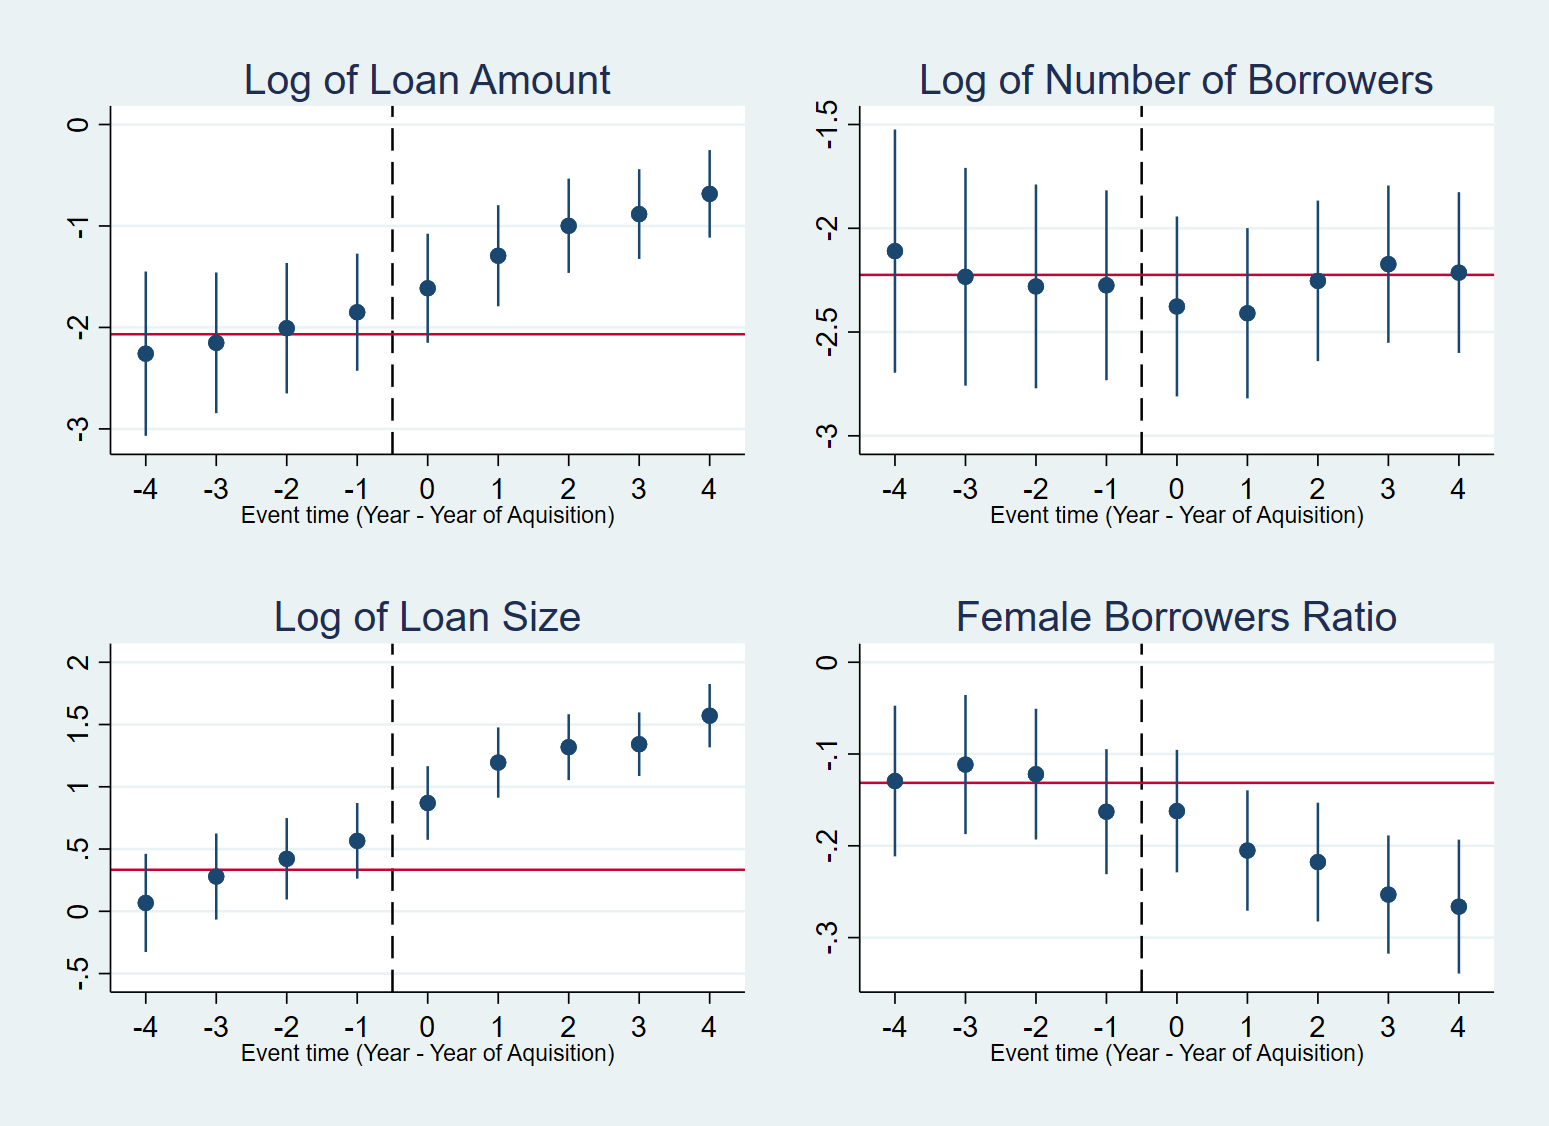
\includegraphics[scale=0.2]{EventStudy.png}
     \\ 
  \footnotesize \raggedright Note: The figure shows the estimated $\beta_{k}$. A red-colored line in each panel represents the average of coefficients before the event.
\end{figure}



Next, we estimated the model of Equation 2, which includes the interaction terms of population density. Figure \ref{figure_Est2} shows the estimated coefficients of interaction terms of population density.  

\begin{figure}[hbtp]
  \centering
  \caption{Coefficients of Interaction terms of Population Density}
  \label{figure_Est2}
  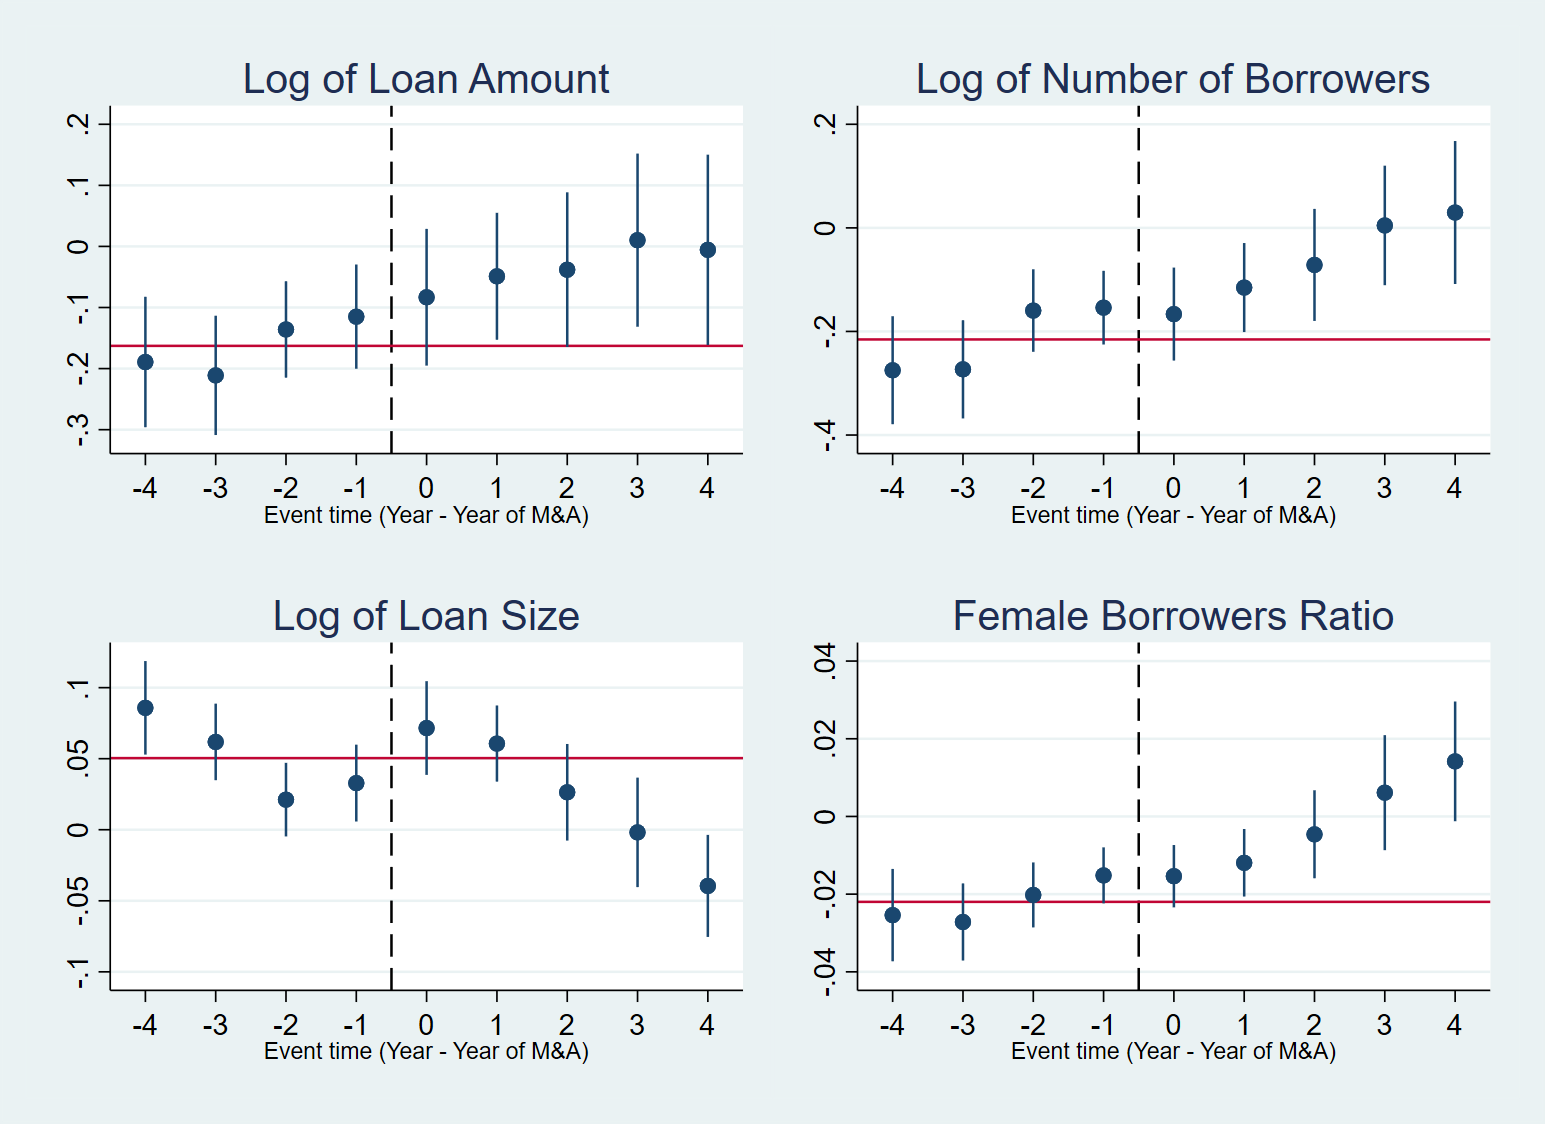
\includegraphics[scale=0.2]{EventStudy2.png}
     \\ 
  \footnotesize \raggedright Note: The figure shows the estimated $\beta_{k}$. A red-colored line in each panel represents the average of coefficients before the event.
\end{figure}


\end{document}